\documentclass[conference]{IEEEtran}
\IEEEoverridecommandlockouts
\usepackage{cite}
\usepackage{amsmath}
\usepackage{graphicx}
\usepackage{booktabs}
\usepackage{multirow}
\usepackage{array}
\usepackage[hyphens]{url}
\usepackage[hidelinks]{hyperref}
\renewcommand{\arraystretch}{1.12}

\begin{document}

\title{Beyond 99\% Accuracy: A Critical Review and Re-evaluation of AI-Based Intrusion Detection for Cloud Environments}

\author{\IEEEauthorblockN{Jayveer Vasava}
\IEEEauthorblockA{\textit{M.Tech (Cyber Security)}\\
\textit{Parul University}\\
Vadodara, Gujarat, India\\
rootjavs@gmail.com}}

\maketitle

\begin{abstract}
AI-based intrusion detection systems (IDS) for cloud environments are routinely reported to exceed 99\% accuracy, yet few of these results are tested under conditions resembling deployment. This paper reviews 30 open-access studies, organised into a taxonomy of classical machine learning, deep learning, hybrid and optimisation methods, feature selection, and explainable and trustworthy AI, and re-evaluates five representative models on the official NSL-KDD and UNSW-NB15 test sets. The best binary F1-scores were 0.798 and 0.897, while a random 80/20 split of the training file alone raised accuracy to 0.998--0.999 and 0.950--0.959. We propose RELIC-IDS, five reliability tests and a 10-point reporting checklist. Unseen attack types were detected at 0.28--0.42 against 0.71--0.79 for known types; false-positive targets fixed on validation data were exceeded 2.2--10 times; class balancing raised rare-class recall only by adding false alarms; and setting the IP time-to-live of attacks to its benign median let 99.8\% of detected UNSW-NB15 attacks evade XGBoost. Finally, we implement RELIC-IDS as an open-source hybrid IDS that combines behaviour rules, a network baseline and a hardened XGBoost model without TTL features. On a scripted capture it detected all four attack scenarios with 6.5\% of normal flows flagged, where the dataset model alone flagged 80\% of normal flows.
\end{abstract}

\begin{IEEEkeywords}
intrusion detection, cloud security, machine learning, evaluation methodology, zero-day attacks, adversarial robustness, explainable AI
\end{IEEEkeywords}

\section{Introduction}
Cloud computing delivers storage, compute and software as on-demand services, and the same properties that make it attractive (multi-tenancy, elastic scaling, virtualised networks and remote access) widen its attack surface. An intrusion detection system (IDS) monitors network traffic or host activity and raises an alert when it observes behaviour that matches an attack or departs from normal operation~\cite{khraisat2019}.

Signature-based IDS match known attack patterns and are precise but blind to new attacks; anomaly-based IDS learn normal behaviour and flag deviations, at the price of false alarms~\cite{khraisat2019,ahmad2021}. In a cloud, traffic volume is high, workloads change constantly, and east--west traffic between virtual machines (VMs) may never cross a perimeter sensor~\cite{nasim2025}. Machine learning (ML) and deep learning (DL) now dominate anomaly-based research, with accuracies often above 99\%. Earlier work warned that ML-based intrusion detection is easy to evaluate optimistically: benchmark datasets are closed worlds, data can leak between training and test sets, and every error is costly in operation~\cite{sommer2010,arp2022}.

This paper asks what lies beyond the 99\% figure. Its contributions are:
\begin{enumerate}
\item a taxonomy and critical review of AI-based IDS for cloud environments built from 30 open-access, verified sources;
\item a reproducible re-evaluation of five models on the official NSL-KDD and UNSW-NB15 test sets that quantifies random-split inflation;
\item RELIC-IDS, five reliability tests (zero-day detection, false-alarm control, rare-class balancing, adversarial mimicry, deployment cost) and a 10-point reporting checklist;
\item an open-source hybrid IDS implementation that acts on these findings, with nine research gaps and matching directions.
\end{enumerate}

\section{Background}
\subsection{Types of intrusion detection}
IDS are classified by method (signature, anomaly or hybrid) and by deployment point: network-based (NIDS) on packets or flows at a virtual switch, flow-log stream or gateway; host-based (HIDS) on system calls and logs of one VM; and hypervisor-based, which can observe inter-VM traffic~\cite{khraisat2019,ahmad2021,nasim2025}.

\subsection{Cloud threat landscape}
Cloud IDS research targets DDoS and resource exhaustion, scanning of tenant address space, credential abuse and insider misuse, malware and botnet traffic, and attacks on the virtualisation layer~\cite{nasim2025,pintoneto2025}. Two properties shape the problem: scale, so training and inference cost matter as much as accuracy; and change, so the notion of normal traffic drifts and a model trained once degrades.

\section{Review Methodology}
The review answered four questions: which AI techniques are used (RQ1), which datasets and metrics evaluate them (RQ2), how well reported results hold under a strict protocol (RQ3), and which gaps remain (RQ4). A seed set of 24 citations from a preliminary survey was checked, and targeted searches were run on IEEE Xplore, arXiv, MDPI, SpringerOpen, Frontiers and CEUR with the terms ``intrusion detection'' AND (``cloud'' OR ``network'') AND (``machine learning'' OR ``deep learning'' OR ``artificial intelligence'' OR ``explainable'' OR ``federated''). Included works had a freely accessible full text and a verifiable record, studied AI-based network or cloud intrusion detection or a dataset used by such studies, and were published 2009--2025. Of the 24 seed citations, 10 could not be verified and 8 lacked free full text or came from low-credibility venues; 6 were retained and 24 were added, giving 30 studies (Fig.~\ref{fig:flow}).

\begin{figure}[t]
\centering
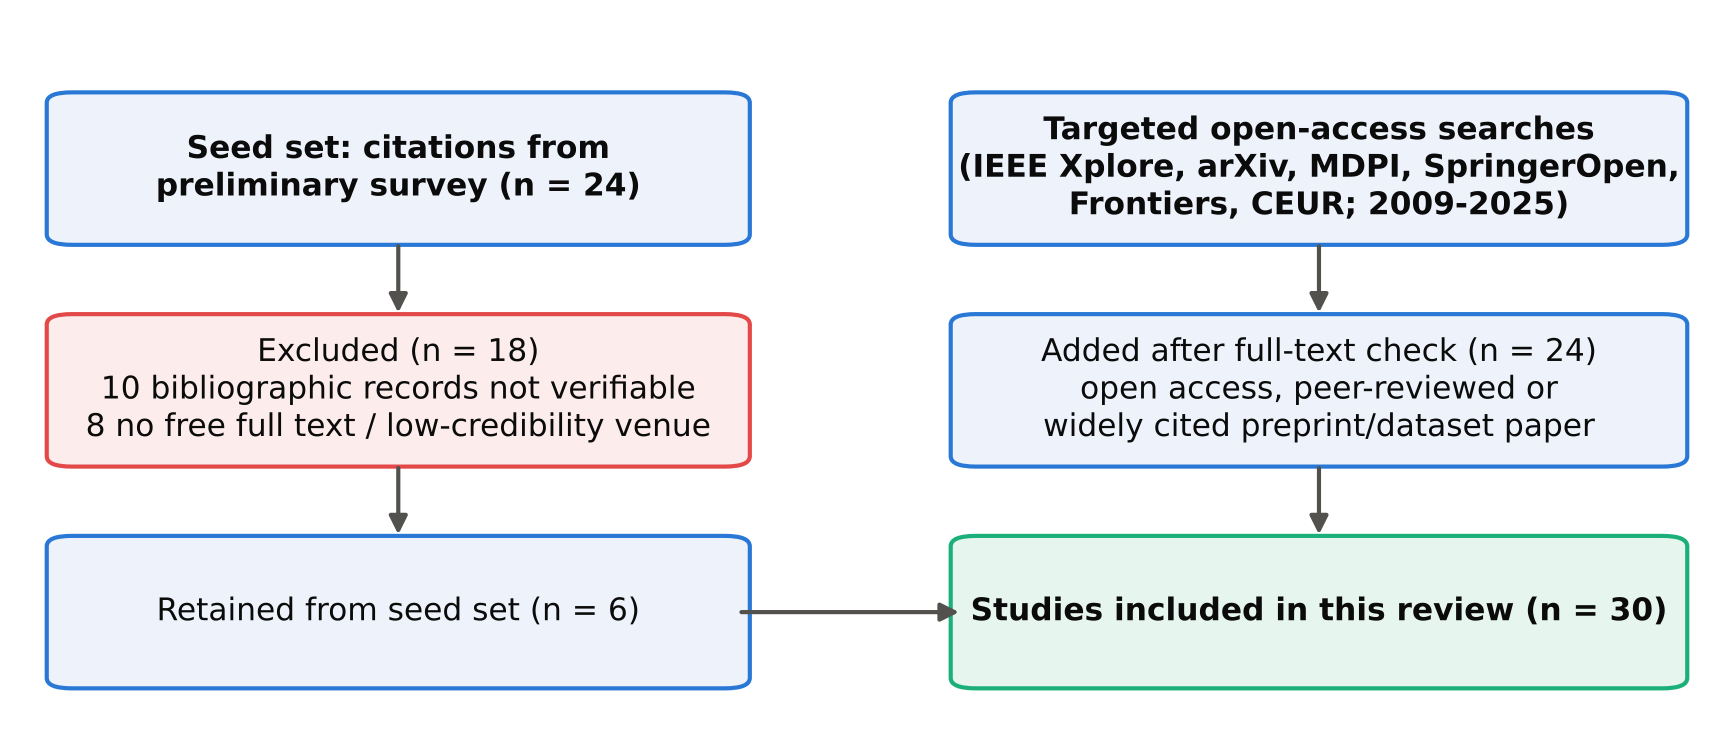
\includegraphics[width=\columnwidth]{figures/fig_selection_flow.png}
\caption{Study selection flow.}
\label{fig:flow}
\end{figure}

\section{Taxonomy of AI Techniques for Cloud IDS}
The studies fall into five overlapping families (Fig.~\ref{fig:tax}). Surveys reach a similar grouping~\cite{pintoneto2025,muneer2024,sharma2024}.

\begin{figure}[t]
\centering
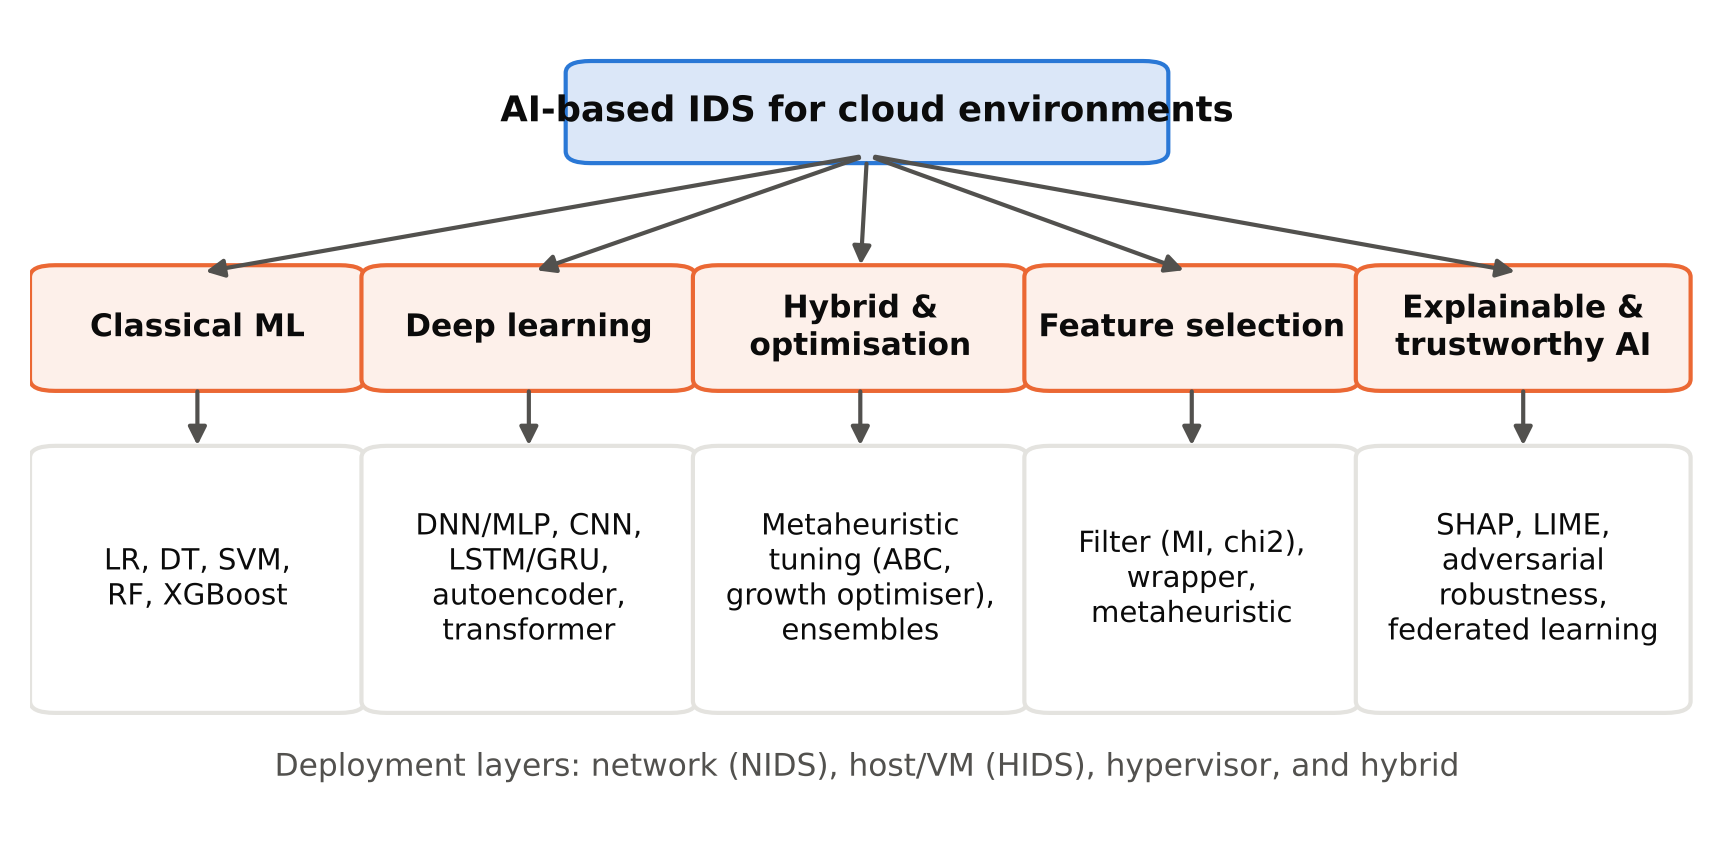
\includegraphics[width=\columnwidth]{figures/fig_taxonomy.png}
\caption{Taxonomy of AI techniques for cloud intrusion detection.}
\label{fig:tax}
\end{figure}

\textit{Classical ML.} Vinayakumar \textit{et al.} compared a deep neural network with classical classifiers on several benchmarks~\cite{vinayakumar2019}. Alzahrani and Alenazi used Decision Tree, Random Forest and XGBoost in an SDN controller, reaching 95.95\% multi-class accuracy on NSL-KDD with 5 of 41 features~\cite{alzahrani2021}. Attou \textit{et al.} report 98.3\% accuracy but 46.0\% recall on NSL-KDD for a Random Forest cloud IDS~\cite{attou2023}, and Maodah \textit{et al.} report close to 100\% accuracy for voting and stacking ensembles~\cite{maodah2025}. XGBoost~\cite{chen2016} is the most common strong baseline.

\textit{Deep learning.} A Transformer encoder reached 93.38--93.46\% on CSE-CIC-IDS2018~\cite{long2024}, and a 1D-CNN with SMOTE reached 98.67\% on the same AWS-generated dataset, with infiltration hardest at 92.43\%~\cite{aljuaid2024}.

\textit{Hybrid and optimisation.} An MLP trained by artificial bee colony with fuzzy clustering was evaluated in CloudSim on NSL-KDD~\cite{hajimirzaei2019}; a later variant reports 99.01\% accuracy and kappa 0.97~\cite{ali2023}.

\textit{Feature selection.} Fatani \textit{et al.} combined CNN feature extraction with a modified Growth Optimizer on four cloud and IoT datasets~\cite{fatani2023}. Rizvi \textit{et al.} measured cost on a constrained VM: Decision Tree and Random Forest reached 99.99\% on IoT-23, but XGBoost used 74.34\% CPU and 587.52\,s of training against 8.26\% and 1.332\,s for a Decision Tree~\cite{rizvi2023,rizvi2022}.

\textit{Explainable and trustworthy AI.} SHAP~\cite{lundberg2017} is the dominant explanation tool~\cite{khan2024,kumar2024}. Federated learning~\cite{agrawal2022}, adversarial robustness~\cite{alhajjar2021} and Transformer or LLM-based IDS~\cite{kheddar2024} extend trustworthiness.

\section{Benchmark Datasets}
Table~\ref{tab:datasets} compares the datasets used by the reviewed studies~\cite{ring2019}. Only CSE-CIC-IDS2018 was generated on cloud infrastructure. NSL-KDD and UNSW-NB15 ship fixed training and test files whose class mix differs: attacks are 46.5\% of NSL-KDD training records but 56.9\% of its test records, and 68.1\% against 55.1\% for UNSW-NB15.

\begin{table}[t]
\caption{Benchmark datasets in the reviewed studies}
\label{tab:datasets}
\centering\scriptsize
\begin{tabular}{@{}>{\raggedright\arraybackslash}p{1.75cm}p{0.55cm}>{\raggedright\arraybackslash}p{2.15cm}>{\raggedright\arraybackslash}p{2.75cm}@{}}
\toprule
Dataset & Year & Size used & Main limitation\\
\midrule
NSL-KDD~\cite{tavallaee2009} & 2009 & 125,973 / 22,544 & 1998 traffic; test-only attack types\\
UNSW-NB15~\cite{moustafa2015} & 2015 & 175,341 / 82,332 & synthetic testbed; tiny classes\\
CICIDS2017~\cite{sharafaldin2018} & 2017 & $\approx$2.8 M flows & heavy class imbalance\\
CSE-CIC-\allowbreak IDS2018~\cite{long2024,aljuaid2024} & 2018 & 12.2 M records~\cite{long2024} & very large; AWS-generated\\
IoT-23~\cite{rizvi2023} & 2020 & varies & IoT, not cloud\\
\bottomrule
\end{tabular}
\end{table}

\section{Comparative Analysis}
Reported accuracies range from 93\% to 100\%, but datasets, splits and metrics differ, so the numbers cannot be ranked (Table~\ref{tab:studies}). Only two studies use cloud-generated traffic~\cite{long2024,aljuaid2024}; accuracy is the headline metric almost everywhere, although~\cite{attou2023} shows 98.3\% accuracy coexisting with 46.0\% recall; and where the protocol is stated, studies evaluate on a random split of one file.

\begin{table}[t]
\caption{Reviewed experimental studies (as reported)}
\label{tab:studies}
\centering\scriptsize
\begin{tabular}{@{}p{0.5cm}>{\raggedright\arraybackslash}p{1.95cm}>{\raggedright\arraybackslash}p{1.7cm}>{\raggedright\arraybackslash}p{1.35cm}>{\raggedright\arraybackslash}p{1.45cm}@{}}
\toprule
Ref. & Model & Dataset & Protocol & Result\\
\midrule
\cite{alzahrani2021} & DT, RF, XGB (5 feat.) & NSL-KDD & multi-class & 95.95\% acc.\\
\cite{attou2023} & RF + feat. eng. & NSL-KDD & not stated & 98.3\% acc., 46.0\% rec.\\
\cite{maodah2025} & voting/stacking & NSL-KDD & not stated & 99.99\% acc.\\
\cite{long2024} & Transformer & CSE-CIC-\allowbreak IDS2018 & random 7:3 & 93.4\% acc.\\
\cite{aljuaid2024} & 1D-CNN + SMOTE & CSE-CIC-\allowbreak IDS2018 & random 70:30 & 98.67\% acc.\\
\cite{hajimirzaei2019} & MLP+ABC+fuzzy & NSL-KDD (CloudSim) & simulation & lower MAE\\
\cite{ali2023} & MLP+ABC+fuzzy & NSL-KDD (CloudSim) & simulation & 99.01\% acc.\\
\cite{fatani2023} & CNN + optimiser & 4 datasets & per dataset & better than baselines\\
\cite{rizvi2023} & 9 ML/DL models & IoT-23 & constrained VM & 99.99\% acc.\\
\bottomrule
\end{tabular}
\end{table}

\section{Experimental Re-evaluation}
\subsection{Setup}
NSL-KDD (KDDTrain+/KDDTest+)~\cite{tavallaee2009} and UNSW-NB15 (official partitions)~\cite{moustafa2015} were used as distributed; no test record was used for training, tuning or scaling. Categorical fields were one-hot encoded (122 and 194 features) and numeric fields standardised, both fitted on training data. Models: Logistic Regression (LR), Decision Tree (DT), Random Forest (RF, 100 trees), XGBoost (200 trees, depth 6)~\cite{chen2016} and an MLP (128--64 units). Binary results are means of three seeds on a 2\,vCPU, 8\,GB cloud container.

\subsection{Binary detection on official test sets}
Table~\ref{tab:binary} shows F1 of 0.742--0.798 on NSL-KDD and 0.849--0.897 on UNSW-NB15. The datasets fail in opposite directions: NSL-KDD precision is 0.92--0.97 but recall 0.62--0.68, while UNSW-NB15 recall is 0.95--0.99 but the false-positive rate (FPR) is 0.25--0.39. The MLP costs 5--16 times more training time than tree models without beating them.

\begin{table}[t]
\caption{Binary detection, official test sets (mean of 3 seeds)}
\label{tab:binary}
\centering\footnotesize
\begin{tabular}{@{}llccccc@{}}
\toprule
Data & Model & Prec. & Rec. & F1 & FPR & AUC\\
\midrule
\multirow{5}{*}{\rotatebox{90}{NSL-KDD}} & LR & 0.917 & 0.623 & 0.742 & 0.074 & 0.792\\
& DT & 0.963 & 0.681 & \textbf{0.798} & 0.034 & 0.823\\
& RF & 0.969 & 0.624 & 0.759 & \textbf{0.027} & 0.960\\
& XGBoost & 0.968 & 0.659 & 0.784 & 0.028 & \textbf{0.965}\\
& MLP & 0.942 & 0.661 & 0.777 & 0.055 & 0.900\\
\midrule
\multirow{5}{*}{\rotatebox{90}{UNSW-NB15}} & LR & 0.753 & 0.972 & 0.849 & 0.391 & 0.956\\
& DT & 0.824 & 0.955 & 0.885 & \textbf{0.250} & 0.855\\
& RF & 0.818 & 0.985 & 0.894 & 0.268 & 0.978\\
& XGBoost & 0.824 & 0.985 & \textbf{0.897} & 0.258 & \textbf{0.984}\\
& MLP & 0.807 & 0.978 & 0.884 & 0.287 & 0.977\\
\bottomrule
\end{tabular}
\end{table}

\subsection{The random-split pitfall}
Training on 80\% of each training file and testing on the remaining 20\% yields 0.998--0.999 accuracy on NSL-KDD against 0.778--0.801 on the official test file, a drop of about 20 points; on UNSW-NB15 the drop is 8--9 points (Fig.~\ref{fig:split}). A random split can place near-duplicate flows from one capture on both sides, so reported results on such splits measure memorisation as much as detection~\cite{sommer2010,arp2022}.

\begin{figure}[t]
\centering
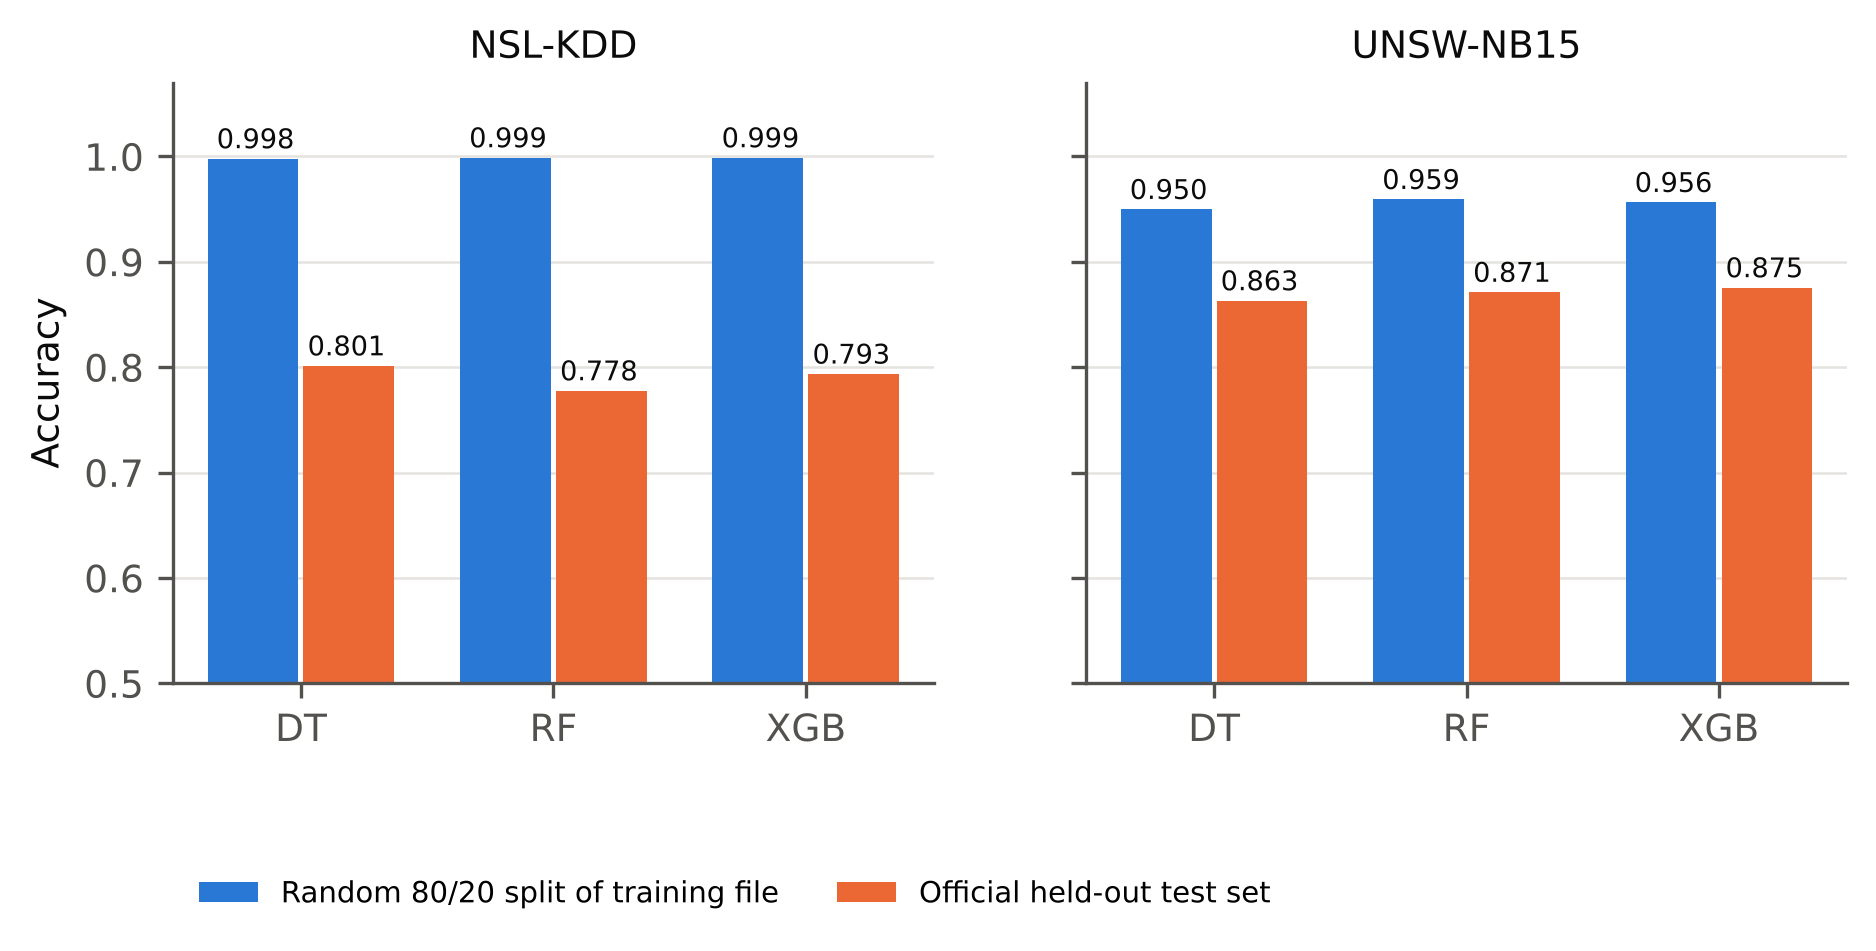
\includegraphics[width=\columnwidth]{figures/fig_split_gap.png}
\caption{Accuracy under a random 80/20 split of the training file versus the official held-out test set.}
\label{fig:split}
\end{figure}

\subsection{Multi-class detection, features and explanations}
Macro-F1 stays at or below 0.564 because rare classes are rarely recognised: the best recall is 0.105 for U2R and 0.112 for R2L on NSL-KDD, and 0.081 for Analysis on UNSW-NB15. Keeping the top 30 features by mutual information cut XGBoost training time by 59\% (NSL-KDD) and 74\% (UNSW-NB15) with an F1 change below 0.01. SHAP~\cite{lundberg2017} on XGBoost shows source bytes dominating on NSL-KDD and a single feature, the source TTL (sttl), dominating on UNSW-NB15 (Fig.~\ref{fig:shap}); a TTL describes the testbed hosts more than the attack.

\begin{figure}[t]
\centering
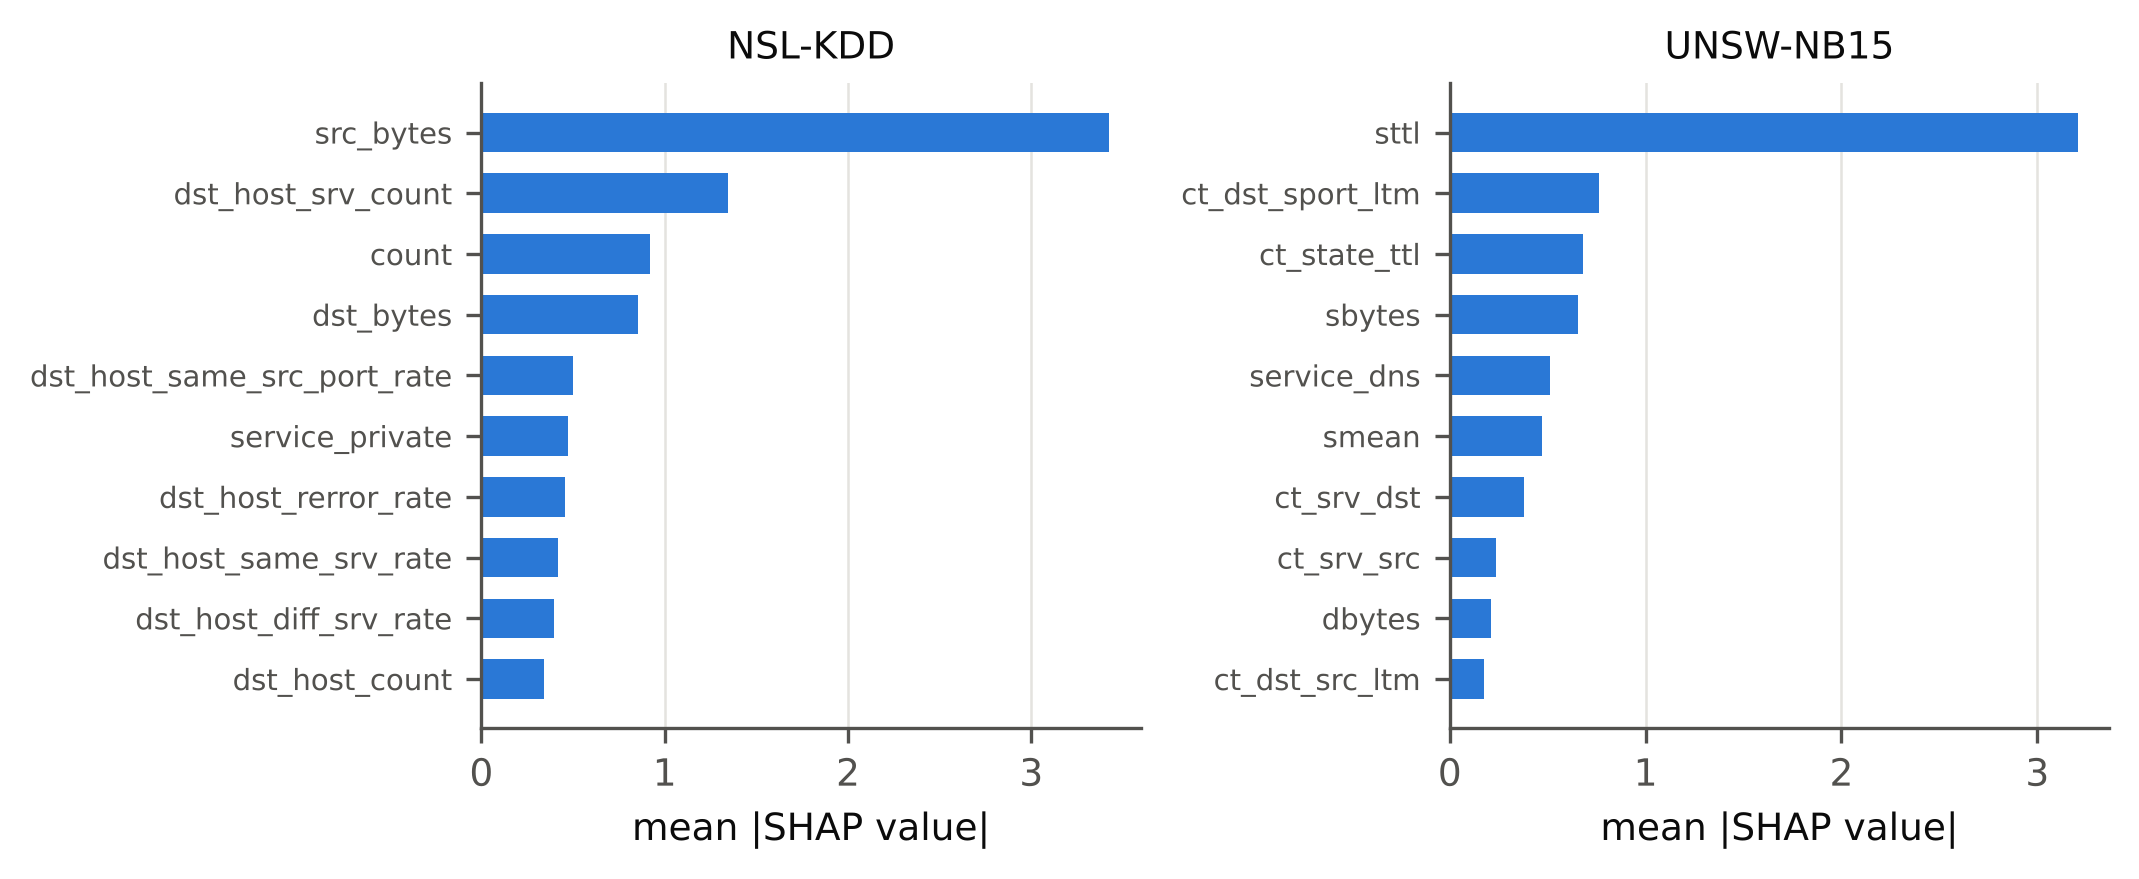
\includegraphics[width=\columnwidth]{figures/fig_shap.png}
\caption{Top-10 features by mean absolute SHAP value (XGBoost).}
\label{fig:shap}
\end{figure}

\section{RELIC-IDS Reliability Tests}
We propose RELIC-IDS (Reliability Evaluation for Learning-based Intrusion detection in Cloud), five tests that each answer an operational question.

\textit{R1, zero-day detection.} The NSL-KDD test file holds 17 attack types (3,750 records) absent from training. Every model detects known types at 0.71--0.79 but unseen types at 0.28--0.42 (Fig.~\ref{fig:zero}); XGBoost missed all 331 snmpguess, 293 mailbomb and 178 snmpgetattack records.

\begin{figure}[t]
\centering
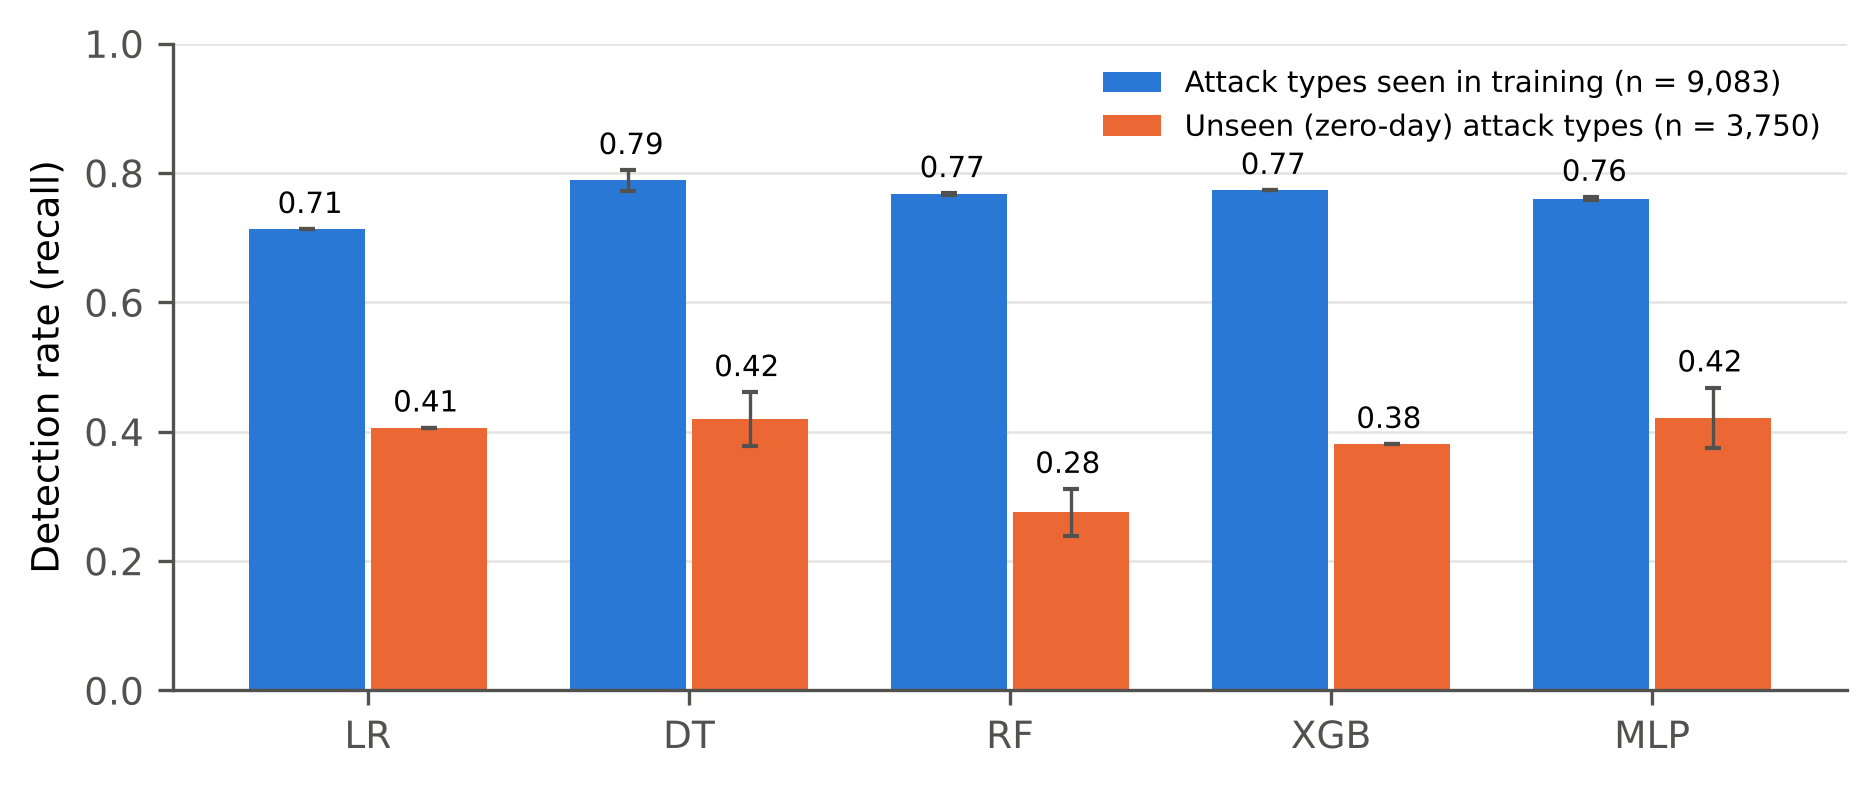
\includegraphics[width=\columnwidth]{figures/fig_zero_day.png}
\caption{Detection of attack types seen in training versus unseen types (NSL-KDD).}
\label{fig:zero}
\end{figure}

\textit{R2, false-alarm control.} Thresholds chosen on a validation split to flag 5\% or 1\% of normal flows were applied to the test set (Table~\ref{tab:thr}). Moving the threshold raised F1 by up to 0.19, but the realised FPR was 2.2--10 times the target, so thresholds need recalibration on production traffic.

\begin{table}[t]
\caption{Validation-set thresholds applied to the official test set}
\label{tab:thr}
\centering\footnotesize
\begin{tabular}{@{}llcccc@{}}
\toprule
Data & Model & Target & Test FPR & Recall & F1\\
\midrule
NSL-KDD & RF & default & 0.027 & 0.603 & 0.743\\
NSL-KDD & RF & 1\% & 0.100 & 0.881 & 0.901\\
NSL-KDD & XGBoost & 1\% & 0.038 & 0.803 & 0.877\\
UNSW-NB15 & RF & 1\% & 0.052 & 0.892 & 0.923\\
UNSW-NB15 & XGBoost & default & 0.259 & 0.986 & 0.897\\
UNSW-NB15 & XGBoost & 1\% & 0.045 & 0.910 & 0.935\\
\bottomrule
\end{tabular}
\end{table}

\textit{R3, rare attacks.} SMOTE doubled NSL-KDD U2R recall to 0.120 (macro-F1 0.581), yet nine in ten U2R and R2L attacks are still missed. On UNSW-NB15, balanced weights raised Backdoor recall from 0.065 to 0.828 but normal recall fell from 0.763 to 0.598, leaving macro-F1 unchanged at 0.507.

\textit{R4, adversarial mimicry.} Detected attacks (8,453 and 44,634) had their top-$k$ SHAP features moved toward the benign median, $x' = (1-\alpha)x + \alpha m$ (Fig.~\ref{fig:adv}). On UNSW-NB15, setting sttl alone to the benign median of 31 (attack median 254) left only 0.19\% of attacks detected; on NSL-KDD, changing the top three features left 11.4\%.

\begin{figure}[t]
\centering
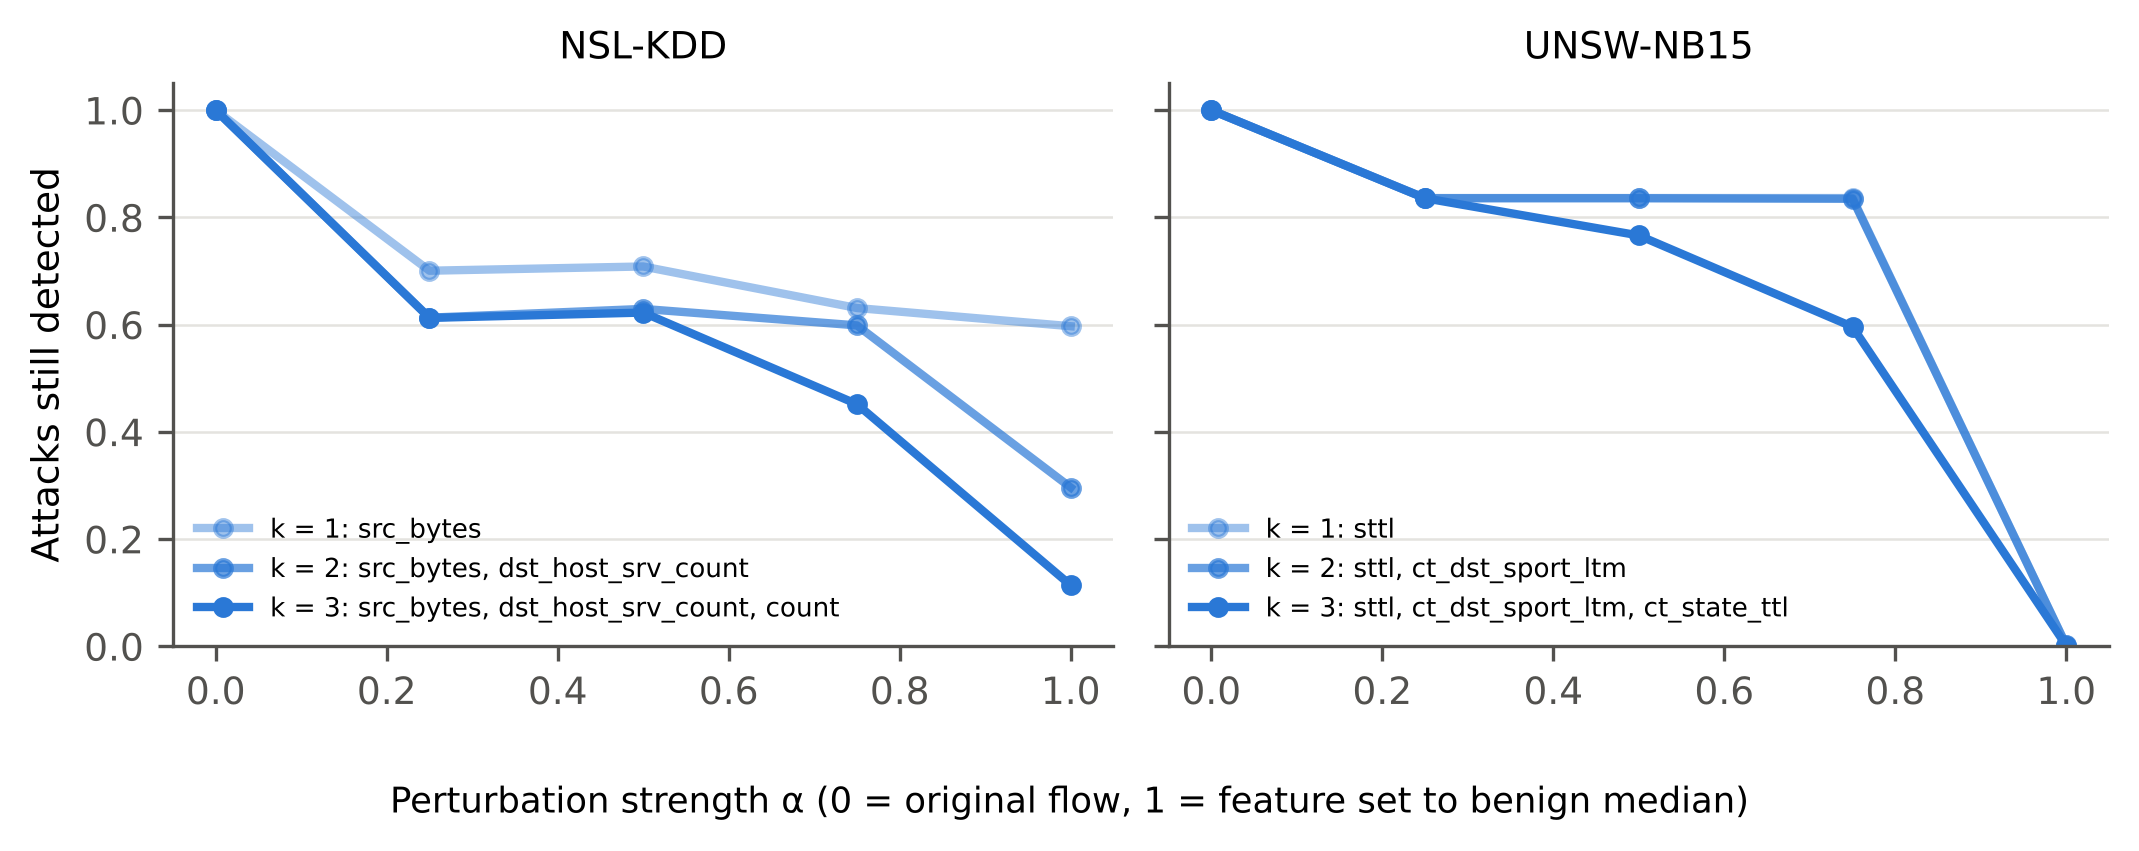
\includegraphics[width=\columnwidth]{figures/fig_adversarial.png}
\caption{Share of detected attacks still detected after their top-$k$ SHAP features are moved toward the benign median (XGBoost).}
\label{fig:adv}
\end{figure}

\textit{R5, deployment cost.} On one CPU thread, XGBoost is 517\,KB with 0.32\,ms latency and 310,120 flows/s; Random Forest is 108\,MB, 6.23\,ms and 121,826 flows/s for a lower F1; LR is 1.4\,KB and 6.2 million flows/s.

\textit{Reporting checklist.} We recommend reporting: (1) results on an official or time-separated test set; (2) mean and spread over at least three seeds; (3) recall, precision, F1, FPR and ROC-AUC; (4) per-class recall; (5) detection of unseen attack types; (6) the threshold and its FPR; (7) balancing and its effect on normal recall; (8) attributions and a robustness check on top features; (9) cost on stated hardware; (10) code and data sufficient to reproduce every number.

\section{RELIC-IDS System Implementation}
The findings above shaped an open-source IDS (Fig.~\ref{fig:system}). A flow builder groups packets from PCAP files or live capture into bidirectional flows and computes 42 UNSW-NB15-style features; its rate, load and inter-packet formulas reproduce official UNSW-NB15 records. Three layers then score every flow. \textit{L1 behaviour rules} detect port scans, host sweeps, SYN, UDP and ICMP floods and brute-force logins from per-host behaviour in time windows. \textit{L2 network baseline} is an Isolation Forest fitted on normal traffic from the protected network, with its threshold set from a chosen false-alarm rate (1\% by default). \textit{L3} is XGBoost trained on UNSW-NB15: a standard 42-feature model for UNSW-format records (F1 0.895) and, following R4, a hardened 35-feature model without TTL and other testbed artefacts for live traffic (F1 0.893, a cost of 0.002). A fusion stage assigns attack type, severity and evidence, groups alerts into incidents, stores runs in SQLite and exports CSV and PDF reports; a Streamlit interface adds SHAP explanations per alert and an attack lab that reproduces R4 interactively.

\begin{figure}[t]
\centering
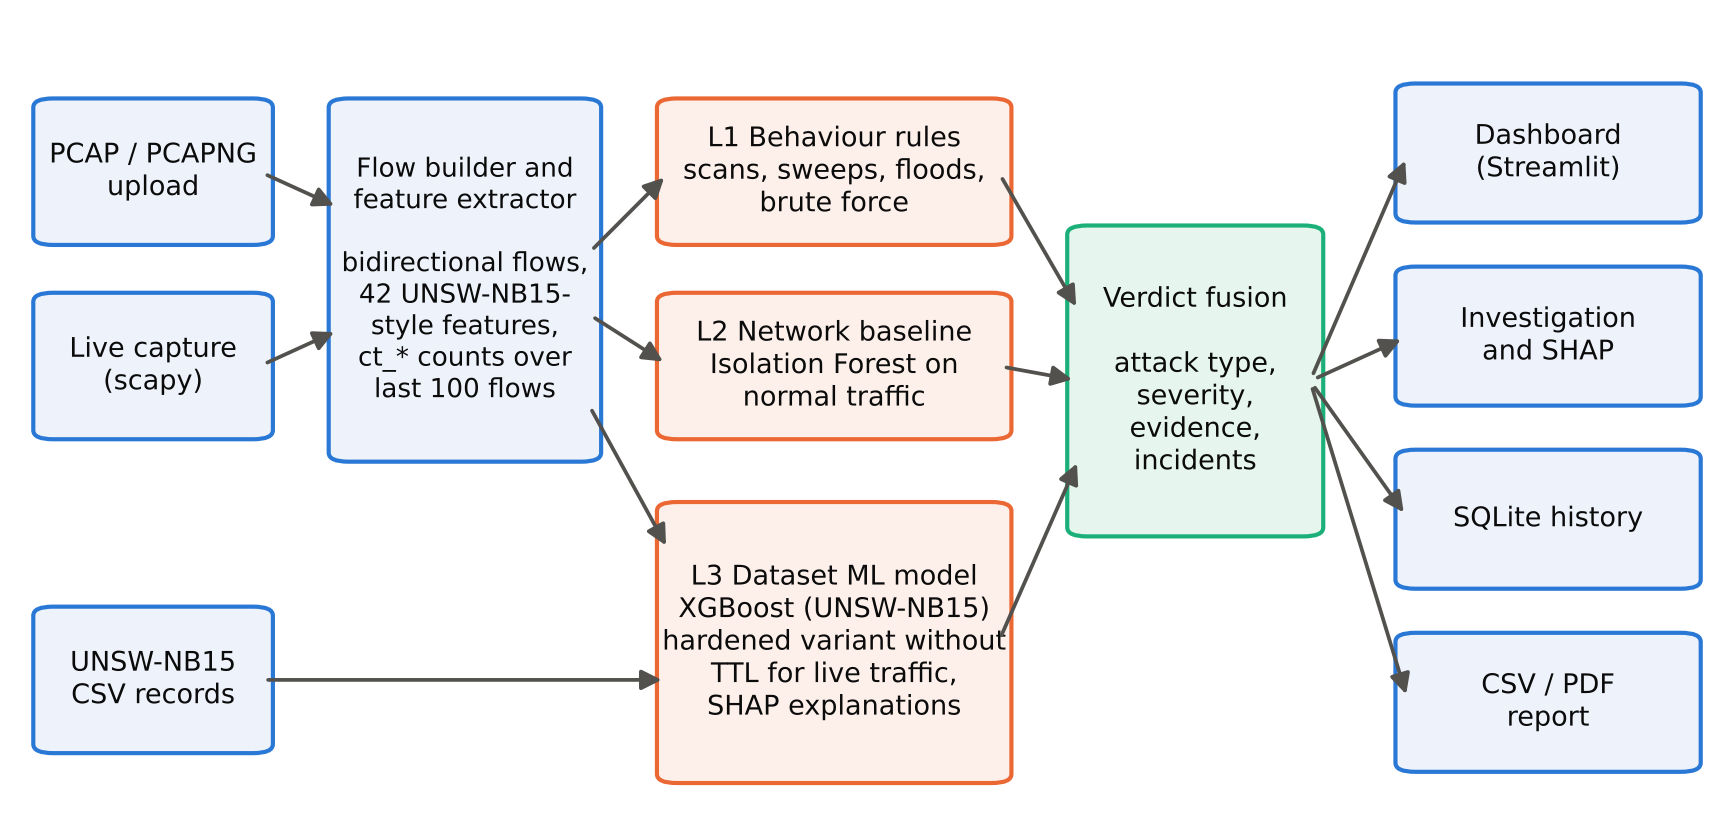
\includegraphics[width=\columnwidth]{figures/fig_system.png}
\caption{Architecture of the RELIC-IDS implementation.}
\label{fig:system}
\end{figure}

We evaluated the system on a scripted two-minute capture of an office network (20 clients using web, DNS and SSH) with a SYN port scan of 1,024 ports, a spoofed SYN flood, a UDP flood and an HTTP brute-force attack, using a separate normal-only capture as baseline. The 8,998 packets became 4,123 flows in about 2\,s. Table~\ref{tab:demo} compares the layers. The lab-trained model alone flagged 80.4\% of normal flows while catching only 2--3\% of scan and flood traffic, a direct measure of dataset shift. The rules caught all four scenarios with no false alarms, and the combined system detected every attack flow with 6.5\% of normal flows flagged as low-severity anomalies. The capture is synthetic and the rule thresholds are standard values, so these numbers demonstrate the design rather than field accuracy.

\begin{table}[t]
\caption{Share of flows flagged on the scripted capture}
\label{tab:demo}
\centering\footnotesize
\begin{tabular}{@{}lrcccc@{}}
\toprule
Scenario & Flows & L3 only & L1 rules & L2 base. & Combined\\
\midrule
Normal & 260 & 0.804 & 0.000 & 0.065 & 0.065\\
Port scan & 1,024 & 0.021 & 1.000 & 1.000 & 1.000\\
DoS floods & 2,689 & 0.025 & 1.000 & 0.441 & 1.000\\
Brute force & 150 & 0.307 & 1.000 & 0.960 & 1.000\\
\bottomrule
\end{tabular}
\end{table}

\section{Research Gaps and Future Directions}
The review and experiments point to nine gaps: (G1) no shared evaluation protocol, with random splits inflating results by 8--20 points; (G2) little cloud-generated data, used by only 2 of 9 experimental studies; (G3) weak detection of unseen attacks; (G4) rare, high-impact attacks missed, with macro-F1 at most 0.58; (G5) uncontrolled false-alarm rates; (G6) explanations produced but rarely acted on, although SHAP exposes artefacts such as sttl; (G7) adversarial robustness rarely tested; (G8) cost seldom reported; and (G9) tenant privacy limiting data sharing~\cite{agrawal2022}.

Matching directions are cloud-native, time-ordered benchmarks in which drift is part of the test; a reporting standard such as the RELIC-IDS checklist; open-set detection that pairs a classifier with an anomaly detector, as in the implementation above; cost-sensitive learning with online threshold recalibration; federated, privacy-preserving training across tenants~\cite{agrawal2022}; robust training under realistic feature constraints~\cite{alhajjar2021}; explanations integrated into analyst workflows~\cite{lundberg2017,khan2024,kumar2024}; Transformer and LLM-assisted detection evaluated under strict protocols~\cite{long2024,kheddar2024}; and lightweight models for the edge--cloud continuum~\cite{rizvi2023}.

\section{Limitations}
NSL-KDD and UNSW-NB15 are laboratory datasets; CSE-CIC-IDS2018 could not be obtained in the experiment environment. Only the MLP represents neural models, and hyperparameters were fixed. The mimicry attack edits feature values rather than packets. Timings come from a shared 2\,vCPU container. The review covers 30 freely accessible studies screened by one reviewer, and the system evaluation uses a synthetic capture.

\section{Conclusion}
Reported 99\% accuracies for AI-based cloud IDS depend heavily on the evaluation protocol. Under official test sets the best F1-scores were 0.798 and 0.897, and the RELIC-IDS tests exposed weaknesses that accuracy hides: unseen attacks detected at about half the rate of known ones, false-alarm targets missed by 2.2--10 times, rare-class gains bought with false alarms, and a single TTL change evading 99.8\% of detections. The implemented hybrid system shows that these findings can be acted on: behaviour rules and a network baseline carry detection on unfamiliar traffic, and a hardened model removes the TTL evasion at negligible cost. Code, data sources and results are available at \url{https://github.com/jayveerv/relic-ids}.

\bibliographystyle{IEEEtran}
\begin{thebibliography}{30}
\bibitem{khraisat2019} A. Khraisat, I. Gondal, P. Vamplew, and J. Kamruzzaman, ``Survey of intrusion detection systems: Techniques, datasets and challenges,'' \textit{Cybersecurity}, vol. 2, art. 20, 2019, doi: 10.1186/s42400-019-0038-7.
\bibitem{ahmad2021} Z. Ahmad, A. S. Khan, C. W. Shiang, J. Abdullah, and F. Ahmad, ``Network intrusion detection system: A systematic study of machine learning and deep learning approaches,'' \textit{Trans. Emerg. Telecommun. Technol.}, vol. 32, no. 1, art. e4150, 2021, doi: 10.1002/ett.4150.
\bibitem{nasim2025} S. S. Nasim, P. Pranav, and S. Dutta, ``A systematic literature review on intrusion detection techniques in cloud computing,'' \textit{Discover Computing}, vol. 28, art. 107, 2025, doi: 10.1007/s10791-025-09641-y.
\bibitem{sommer2010} R. Sommer and V. Paxson, ``Outside the closed world: On using machine learning for network intrusion detection,'' in \textit{Proc. IEEE Symp. Security and Privacy}, 2010, pp. 305--316, doi: 10.1109/SP.2010.25.
\bibitem{arp2022} D. Arp \textit{et al.}, ``Dos and don'ts of machine learning in computer security,'' in \textit{Proc. 31st USENIX Security Symp.}, 2022, arXiv:2010.09470.
\bibitem{pintoneto2025} E. C. Pinto Neto, S. Iqbal, S. Buffett, M. Sultana, and A. Taylor, ``Deep learning for intrusion detection in emerging technologies: A comprehensive survey and new perspectives,'' \textit{Artif. Intell. Rev.}, vol. 58, no. 10, art. 340, 2025, doi: 10.1007/s10462-025-11346-z.
\bibitem{muneer2024} S. Muneer, U. Farooq, A. Athar, M. A. Raza, T. M. Ghazal, and S. Sakib, ``A critical review of artificial intelligence based approaches in intrusion detection: A comprehensive analysis,'' \textit{J. Eng.}, vol. 2024, art. 3909173, 2024, doi: 10.1155/2024/3909173.
\bibitem{sharma2024} V. Sharma, D. Shah, S. Sharma, and S. Gautam, ``Artificial intelligence based intrusion detection system---A detailed survey,'' \textit{ITM Web Conf.}, vol. 65, art. 04002, 2024, doi: 10.1051/itmconf/20246504002.
\bibitem{vinayakumar2019} R. Vinayakumar, M. Alazab, K. P. Soman, P. Poornachandran, A. Al-Nemrat, and S. Venkatraman, ``Deep learning approach for intelligent intrusion detection system,'' \textit{IEEE Access}, vol. 7, pp. 41525--41550, 2019, doi: 10.1109/ACCESS.2019.2895334.
\bibitem{alzahrani2021} A. O. Alzahrani and M. J. F. Alenazi, ``Designing a network intrusion detection system based on machine learning for software defined networks,'' \textit{Future Internet}, vol. 13, no. 5, art. 111, 2021, doi: 10.3390/fi13050111.
\bibitem{attou2023} H. Attou, A. Guezzaz, S. Benkirane, M. Azrour, and Y. Farhaoui, ``Cloud-based intrusion detection approach using machine learning techniques,'' \textit{Big Data Mining and Analytics}, vol. 6, no. 3, pp. 311--320, 2023, doi: 10.26599/BDMA.2022.9020038.
\bibitem{maodah2025} K. A. Maodah, S. Alhomdy, and F. Thabit, ``Detecting intrusions in cloud-based ensembles: Evaluating voting and stacking methods with machine learning classifiers,'' \textit{Front. Comput. Sci.}, vol. 7, art. 1623375, 2025, doi: 10.3389/fcomp.2025.1623375.
\bibitem{chen2016} T. Chen and C. Guestrin, ``XGBoost: A scalable tree boosting system,'' in \textit{Proc. 22nd ACM SIGKDD Int. Conf. Knowledge Discovery and Data Mining}, 2016, pp. 785--794.
\bibitem{long2024} Z. Long, H. Yan, G. Shen, X. Zhang, H. He, and L. Cheng, ``A Transformer-based network intrusion detection approach for cloud security,'' \textit{J. Cloud Comput.}, vol. 13, art. 5, 2024, doi: 10.1186/s13677-023-00574-9.
\bibitem{aljuaid2024} W. H. Aljuaid and S. S. Alshamrani, ``A deep learning approach for intrusion detection systems in cloud computing environments,'' \textit{Appl. Sci.}, vol. 14, no. 13, art. 5381, 2024, doi: 10.3390/app14135381.
\bibitem{hajimirzaei2019} B. Hajimirzaei and N. J. Navimipour, ``Intrusion detection for cloud computing using neural networks and artificial bee colony optimization algorithm,'' \textit{ICT Express}, vol. 5, no. 1, pp. 56--59, 2019, doi: 10.1016/j.icte.2018.01.014.
\bibitem{ali2023} M. Ali, A. Razaque, D. M. Yeskendirova, T. A. Nurlybayev, N. Y. Askarbekova, and Z. A. Kashaganova, ``Enhancing cloud computing security through AI-based intelligent intrusion detection leveraging neural networks and artificial bee colony optimization,'' in \textit{Proc. DTESI}, CEUR Workshop Proc., vol. 3680, 2023.
\bibitem{fatani2023} A. Fatani \textit{et al.}, ``Enhancing intrusion detection systems for IoT and cloud environments using a growth optimizer algorithm and conventional neural networks,'' \textit{Sensors}, vol. 23, no. 9, art. 4430, 2023, doi: 10.3390/s23094430.
\bibitem{rizvi2023} S. Rizvi, M. Scanlon, J. McGibney, and J. Sheppard, ``An evaluation of AI-based network intrusion detection in resource-constrained environments,'' in \textit{Proc. IEEE 14th UEMCON}, 2023.
\bibitem{rizvi2022} S. Rizvi, M. Scanlon, J. McGibney, and J. Sheppard, ``Application of artificial intelligence to network forensics: Survey, challenges and future directions,'' \textit{IEEE Access}, vol. 10, pp. 110362--110384, 2022, doi: 10.1109/ACCESS.2022.3214506.
\bibitem{lundberg2017} S. M. Lundberg and S.-I. Lee, ``A unified approach to interpreting model predictions,'' in \textit{Advances in Neural Information Processing Systems 30}, 2017.
\bibitem{khan2024} N. Khan, K. Ahmad, A. Al Tamimi, M. M. Alani, A. Bermak, and I. Khalil, ``Explainable AI-based intrusion detection system for Industry 5.0: An overview of the literature, associated challenges, the existing solutions, and potential research directions,'' 2024, arXiv:2408.03335.
\bibitem{kumar2024} A. Kumar and V. L. L. Thing, ``Evaluating the explainability of state-of-the-art machine learning-based IoT network intrusion detection systems,'' 2024, arXiv:2408.14040.
\bibitem{agrawal2022} S. Agrawal \textit{et al.}, ``Federated learning for intrusion detection system: Concepts, challenges and future directions,'' \textit{Comput. Commun.}, vol. 195, pp. 346--361, 2022.
\bibitem{alhajjar2021} E. Alhajjar, P. Maxwell, and N. Bastian, ``Adversarial machine learning in network intrusion detection systems,'' \textit{Expert Syst. Appl.}, vol. 186, art. 115782, 2021.
\bibitem{kheddar2024} H. Kheddar, ``Transformers and large language models for efficient intrusion detection systems: A comprehensive survey,'' 2024, arXiv:2408.07583.
\bibitem{ring2019} M. Ring, S. Wunderlich, D. Scheuring, D. Landes, and A. Hotho, ``A survey of network-based intrusion detection data sets,'' \textit{Comput. Secur.}, vol. 86, pp. 147--167, 2019.
\bibitem{tavallaee2009} M. Tavallaee, E. Bagheri, W. Lu, and A. A. Ghorbani, ``A detailed analysis of the KDD CUP 99 data set,'' in \textit{Proc. IEEE CISDA}, 2009, pp. 1--6, doi: 10.1109/CISDA.2009.5356528.
\bibitem{moustafa2015} N. Moustafa and J. Slay, ``UNSW-NB15: A comprehensive data set for network intrusion detection systems,'' in \textit{Proc. MilCIS}, 2015, pp. 1--6, doi: 10.1109/MilCIS.2015.7348942.
\bibitem{sharafaldin2018} I. Sharafaldin, A. H. Lashkari, and A. A. Ghorbani, ``Toward generating a new intrusion detection dataset and intrusion traffic characterization,'' in \textit{Proc. 4th ICISSP}, 2018, pp. 108--116, doi: 10.5220/0006639801080116.
\end{thebibliography}

\end{document}
